
\bta{2015}



\section{Use of English}

\noindent
\textbf{Directions:}\\
{Read the following text. Choose the best word (s) for each
	numbered blank and mark A, B, C or D on \textbf{ANSWER SHEET 1}. (10 points)}


\TiGanSpace


Though not biologically related, friends are as ``related'' as fourth
cousins, sharing about 1\% of genes. That is \cloze a
study, published from the University of California and Yale University in
the Proceedings of the National Academy of Sciences, has \cloze .

The study is a genome-wide analysis conducted \cloze 1932 unique
subjects which \cloze pairs of unrelated friends and unrelated
strangers. The same people were used in both \cloze.

While 1\% may seem \cloze , it is not so to a geneticist. As
co-author of the study James Fowler, professor of medical genetics at UC
San Diego, says, " Most people do not even \cloze their fourth
cousins but somehow manage to select as friends the people who
\cloze our kin."

The study \cloze found that the genes for smell were something
shared in friends but not genes for immunity. Why this similarity exists
in smell genes is difficult to explain, for now. \cloze , as the
team suggests, it draws us to similar environments but there is more
\cloze it. There could be many mechanisms working together that
\cloze us in choosing genetically similar friends \cloze
``functional kinship'' of being friends with \cloze !

One of the remarkable findings of the study was that the similar genes
seem to be evolving \cloze than other genes. Studying this could
help \cloze why human evolution picked pace in the last 30, 000
years, with social environment being a major \cloze factor.

The findings do not simply explain people's \cloze to befriend
those of similar \cloze backgrounds, say the researchers. Though
all the subjects were drawn from a population of European extraction,
care was taken to \cloze that all subjects, friends and strangers
were taken from the same population.


\newpage
\begin{enumerate}
	%\renewcommand{\labelenumi}{\arabic{enumi}.}
	% A(\Alph) a(\alph) I(\Roman) i(\roman) 1(\arabic)
	%设定全局标号series=example	%引用全局变量resume=example
	%[topsep=-0.3em,parsep=-0.3em,itemsep=-0.3em,partopsep=-0.3em]
	%可使用leftmargin调整列表环境左边的空白长度 [leftmargin=0em]
	\item

\fourchoices
{when}
{why}
{how}
{what}




\item


\fourchoices
{defended}
{concluded}
{withdrawn}
{advised}




\item


\fourchoices
{for}
{with}
{on}
{by}




\item


\fourchoices
{compared}
{sought}
{separated}
{connected}




\item


\fourchoices
{tests}
{objects}
{samples}
{examples}




\item

\fourchoices
{insignificant}
{unexpected}
{unreliable}
{incredible}



\item


\fourchoices
{visit}
{miss}
{seek}
{know}




\item


\fourchoices
{resemble}
{influence}
{favor}
{surpass}




\item


\fourchoices
{again}
{also}
{instead}
{thus}




\item

\fourchoices
{Meanwhile}
{Furthermore}
{Likewise}
{Perhaps}



\item


\fourchoices
{about}
{to}
{from}
{like}




\item


\fourchoices
{drive}
{observe}
{confuse}
{limit}




\item

\fourchoices
{according to}
{rather than}
{regardless of}
{along with}


\item


\fourchoices
{chances}
{responses}
{missions}
{benefits}




\item


\fourchoices
{later}
{slower}
{faster}
{earlier}




\item


\fourchoices
{forecast}
{remember}
{understand}
{express}




\item

\fourchoices
{unpredictable}
{contributory}
{controllable}
{disruptive}


\item

\fourchoices
{endeavor}
{decision}
{arrangement}
{tendency}



\item


\fourchoices
{political}
{religious}
{ethnic}
{economic}




\item


\fourchoices
{see}
{show}
{prove}
{tell}

\end{enumerate}

\vfil

\section{Reading Comprehension}


\noindent
\textbf{Part A}\\
\textbf{Directions:}\\
Read the following four texts. Answer the questions below each
	text by choosing A, B, C or
	D. Mark your answers on the \textbf{ANSWER SHEET 1}.
	(40 points)

\newpage
\subsection{Text 1}


King Juan Carlos of Spain once insisted ``kings don't abdicate, they die
in their sleep.'' But embarrassing scandals and the popularity of the
republican left in the recent Euro-elections have forced him to eat his
words and stand down. So, does the Spanish crisis suggest that monarchy
is seeing its last days? Does that mean the writing is on the wall for
all European royals, with their magnificent uniforms and majestic
lifestyles?

The Spanish case provides arguments both for and against monarchy. When
public opinion is particularly polarised, as it was following the end of
the Franco regime, monarchs can rise above ``mere'' politics and
``embody'' a spirit of national unity.

It is this apparent transcendence of politics that explains monarchs'
continuing popularity as heads of state. And so, the Middle East
excepted, Europe is the most monarch-infested region in the world, with
10 kingdoms (not counting Vatican City and Andorra). But unlike their
absolutist counterparts in the Gulf and Asia, most royal families have
survived because they allow voters to avoid the difficult search for a
non-controversial but respected public figure.

Even so, kings and queens undoubtedly have a downside. Symbolic of
national unity as they claim to be, their very history---and sometimes
the way they behave today---embodies outdated and indefensible
privileges and inequalities. At a time when Thomas Piketty and other
economists are warning of rising inequality and the increasing power of
inherited wealth, it is bizarre that wealthy aristocratic families
should still be the symbolic heart of modern democratic states.

The most successful monarchies strive to abandon or hide their old
aristocratic ways. Princes and princesses have day-jobs and ride
bicycles, not horses (or helicopters). Even so, these are wealthy
families who party with the international 1\%, and media intrusiveness
makes it increasingly difficult to maintain the right image.

While Europe's monarchies will no doubt be smart enough to survive for
some time to come, it is the British royals who have most to fear from
the Spanish example.

It is only the Queen who has preserved the monarchy's reputation with
her rather ordinary (if well-heeled) granny style. The danger will come
with Charles, who has both an expensive taste of lifestyle and a pretty
hierarchical view of the world. He has failed to understand that
monarchies have largely survived because they provide a service---as
non-controversial and non-political heads of state. Charles ought to
know that as English history shows, it is kings, not republicans, who
are the monarchy's worst enemies.


\begin{enumerate}[resume]
	%\renewcommand{\labelenumi}{\arabic{enumi}.}
	% A(\Alph) a(\alph) I(\Roman) i(\roman) 1(\arabic)
	%设定全局标号series=example	%引用全局变量resume=example
	%[topsep=-0.3em,parsep=-0.3em,itemsep=-0.3em,partopsep=-0.3em]
	%可使用leftmargin调整列表环境左边的空白长度 [leftmargin=0em]
	\item
 According to the first two Paragraphs, King Juan
	Carlosof Spain \lineread.


\fourchoices
{used to enjoy high public support}
{was unpopular among European royals}
{eased his relationship with his rivals}
{ended his reign in embarrassment}


\item
 Monarchs are kept as heads of state in Europe
mostly \lineread.


\fourchoices
{owing to their undoubted and respectable status}
{to achieve a balance between tradition and reality}
{to give voters more public figures to look up to}
{due to their everlasting political embodiment}



\item
Which of the following is shown to be odd, according to
Paragraph 4?


\fourchoices
{Aristocrats' excessive reliance on inherited wealth.}
{The role of the nobility in modern democracies.}
{The simple lifestyle of the aristocratic families.}
{The nobility's adherence to their privileges.}


\item
The British royals ``have most to fear'' because
Charles \lineread.


\fourchoices
{takes a tough line on political issues}
{fails to change his lifestyle as advised}
{takes republicans as his potential allies}
{fails to adapt himself to his future role}



\item
Which of the following is the best title of the text?


\fourchoices
{Carlos, Glory and Disgrace Combined}
{Charles, Anxious to Succeed to the Throne}
{Carlos, a Lesson for All European Monarchs}
{Charles, Slow to React to the Coming Threats}


\end{enumerate}


\newpage
\subsection{Text 2}


Just how much does the Constitution protect your digital data? The
Supreme Court will now consider whether police can search the contents
of a mobile phone without a warrant if the phone is on or around a
person during an arrest.

California has asked the justices to refrain from a sweeping ruling,
particularly one that upsets the old assumption that authorities may
search through the possessions of suspects at the time of their arrest.
It is hard, the state argues, for judges to assess the implications of
new and rapidly changing technologies.

The court would be recklessly modest if it followed California's advice.
Enough of the implications are discernable, even obvious, so that the
justices can and should provide updated guidelines to police, lawyers and
defendants.

They should start by discarding California's lame argument that
exploring the contents of a smartphone---a vast storehouse of digital
information---is similar to, say, going through a suspect's purse. The
court has ruled that police don't violate the Fourth Amendment when they
go through the wallet or pocketbook of an arrestee without a warrant.
But exploring one's smartphone is more like entering his or her home. A
smartphone may contain an arrestee's reading history, financial history,
medical history and comprehensive records of recent correspondence. The
development of ``cloud computing,'' meanwhile, has made that exploration
so much the easier.

Americans should take steps to protect their digital privacy. But
keeping sensitive information on these devices is increasingly a
requirement of normal life. Citizens still have a right to expect
private documents to remain private and protected by the Constitution's
prohibition on unreasonable searches.

As so often is the case, stating that principle doesn't ease the
challenge of line-drawing. In many cases, it would not be overly
burdensome for authorities to obtain a warrant to search through phone
contents. They could still invalidate Fourth Amendment protections when
facing severe, urgent circumstances, and they could take reasonable
measures to ensure that phone data are not erased or altered while
waiting for a warrant. The court, though, may want to allow room for
police to cite situations where they are entitled to more freedom.

But the justices should not swallow California's argument whole. New,
disruptive technology sometimes demands novel applications of the
Constitution's protections. Orin Kerr, a law professor, compares the
explosion and accessibility of digital information in the 21st century
with the establishment of automobile use as a virtual necessity of life
in the 20th: The justices had to specify novel rules for the new
personal domain of the passenger car then; they must sort out how the
Fourth Amendment applies to digital information now.


\begin{enumerate}[resume]
	%\renewcommand{\labelenumi}{\arabic{enumi}.}
	% A(\Alph) a(\alph) I(\Roman) i(\roman) 1(\arabic)
	%设定全局标号series=example	%引用全局变量resume=example
	%[topsep=-0.3em,parsep=-0.3em,itemsep=-0.3em,partopsep=-0.3em]
	%可使用leftmargin调整列表环境左边的空白长度 [leftmargin=0em]
	\item
The Supreme Court will work out whether, during an arrest,
it is legitimate to \lineread.


\fourchoices
{prevent suspects from deleting their phone contents}
{search for suspects' mobile phones without a warrant}
{check suspects' phone contents without being authorized}
{prohibit suspects from using their mobile phones}


\item
The author's attitude toward California's argument is one
of \lineread.


\fourchoices
{disapproval}
{indifference}
{tolerance}
{cautiousness}



\item
The author believes that exploring one's phone contents is
comparable to \lineread.


\fourchoices
{getting into one's residence}
{handling one's historical records}
{scanning one's correspondences}
{going through one's wallet}



\item
 In Paragraph 5 and 6, the author shows his concern
that \lineread.


\fourchoices
{principles are hard to be clearly expressed}
{the court is giving police less room for action}
{citizens' privacy is not effectively protected}
{phones are used to store sensitive information}


\item
Orin Kerr's comparison is quoted to indicate
that \lineread.


\fourchoices
{the Constitution should be implemented flexibly}
{new technology requires reinterpretation of the Constitution}
{California's argument violates principles of the Constitution}
{principles of the Constitution should never be altered}


\end{enumerate}



\newpage
\subsection{Text 3}


The journal Science is adding an extra round of statistical checks to
its peer-review process, editor-in-chief Marcia McNutt announced today.
The policy follows similar efforts from other journals, after widespread
concern that basic mistakes in data analysis are contributing to the
irreproducibility of many published research findings.

``Readers must have confidence in the conclusions published in our
journal,'' writes McNutt in an editorial. Working with the American
Statistical Association, the journal has appointed seven experts to a
statistic board of reviewing editors (SBoRE). Manuscript will be
\uline{flagged up} for additional scrutiny by the journal's internal
editors, or by its existing Board of Reviewing Editors or by outside
peer reviewers. The SBoRE panel will then find external statisticians to
review these manuscripts.

Asked whether any particular papers had impelled the change, McNutt
said: ``The creation of the `statistics board' was motivated by concerns
broadly with the application of statistics and data analysis in
scientific research and is part of Science's overall drive to increase
reproducibility in the research we publish.''

Giovanni Parmigiani, a biostatistician at the Harvard School of Public
Health, a member of the SBoRE group, says he expects the board to ``play
primarily an advisory role.'' He agreed to join because he ``found the
foresight behind the establishment of the SBoRE to be novel, unique and
likely to have a lasting impact. This impact will not only be through
the publications in Science itself, but hopefully through a larger group
of publishing places that may want to model their approach
after \emph{Science}.''

John Ioannidis, a physician who studies research methodology, says that
the policy is ``a most welcome step forward'' and ``long overdue.''
``Most journals are weak in statistical review, and this damages the
quality of what they publish. I think that, for the majority of
scientific papers nowadays, statistical review is more essential than
expert review,'' he says. But he noted that biomedical journals such as
\emph{Annals of Internal Medicine, the Journal of the American Medical
Association} and \emph{The Lancet} pay strong attention to statistical review.

Professional scientists are expected to know how to analyze data, but
statistical errors are alarmingly common in published research,
according to David Vaux, a cell biologist. Researchers should improve
their standards, he wrote in 2012, but journals should also take a
tougher line, ``engaging reviewers who are statistically literate and
editors who can verify the process.'' Vaux says that Science's idea to
pass some papers to statisticians ``has some merit, but a weakness is
that it relies on the board of reviewing editors to identify `the papers
that need scrutiny' in the first place''.


\begin{enumerate}[resume]
	%\renewcommand{\labelenumi}{\arabic{enumi}.}
	% A(\Alph) a(\alph) I(\Roman) i(\roman) 1(\arabic)
	%设定全局标号series=example	%引用全局变量resume=example
	%[topsep=-0.3em,parsep=-0.3em,itemsep=-0.3em,partopsep=-0.3em]
	%可使用leftmargin调整列表环境左边的空白长度 [leftmargin=0em]
	\item
It can be learned from Paragraph 1 that \lineread.


\fourchoices
{\emph{Science} intends to simplify its peer-review process}
{journals are strengthening their statistical checks}
{few journals are blamed for mistakes in data analysis}
{lack of data analysis is common in research projects}


\item
The phrase ``flagged up'' (Para. 2) is the closest in
meaning to \lineread.



\fourchoices
{found}
{marked}
{revised}
{stored}




\item
Giovanni Parmigiani believes that the establishment of the
SBoRE may \lineread.


\fourchoices
{pose a threat to all its peers}
{meet with strong opposition}
{increase \emph{Science}'s circulation}
{set an example for other journals}



\item
 David Vaux holds that what \emph{Science} is doing
	now \lineread.


\fourchoices
{adds to researchers' workload}
{diminishes the role of reviewers}
{has room for further improvement}
{is to fail in the foreseeable future}



\item
Which of the following is the best title of the text?


\fourchoices
{\emph{Science} Joins Push to Screen Statistics in Papers}
{Professional Statisticians Deserve More Respect}
{Data Analysis Finds Its Way onto Editors' Desks}
{Statisticians Are Coming Back with \emph{Science}}


\end{enumerate}


\newpage
\subsection{Text 4}


Two years ago, Rupert Murdoch's daughter, Elisabeth, spoke of the
``unsettling dearth of integrity across so many of our institutions.''
Integrity had collapsed, she argued, because of a collective acceptance
that the only ``sorting mechanism'' in society should be profit and the
market. But ``it's us, human beings, we the people who create the
society we want, not profit''.

Driving her point home, she continued: ``It's increasingly apparent that
the absence of purpose, of a moral language within government, media or
business could become one of the most dangerous goals for capitalism and
freedom.'' This same absence of moral purpose was wounding companies
such as News International, she thought, making it more likely that it
would lose its way as it had with widespread illegal telephone hacking.

As the hacking trial concludes---finding guilty one ex-editor of
the \emph{News of the World}, Andy Coulson, for conspiring to hack
phones, and finding his predecessor, Rebekah Brooks, innocent of the
same charge---the wider issue of dearth of integrity still
stands. Journalists are known to have hacked the phones of up to 5, 500
people. This is hacking on an industrial scale, as was acknowledged by
Glenn Mulcaire, the man hired by the \emph{News of the World} in 2001 to
be the point person for phone hacking. Others await trial. This long
story still unfolds.

In many respects, the dearth of moral purpose frames not only the fact
of such widespread phone hacking but the terms on which the trial took
place. One of the astonishing revelations was how little Rebekah Brooks
knew of what went on in her newsroom, how little she thought to ask and
the fact that she never inquired how the stories arrived. The core of
her successful defence was that she knew nothing.

In today's world, it has become normal that well-paid executives should
not be accountable for what happens in the organizations that they run.
Perhaps we should not be so surprised. For a generation, the collective
doctrine has been that the sorting mechanism of society should be
profit. The words that have mattered are efficiency, flexibility,
shareholder value, business--friendly, wealth generation, sales, impact
and, in newspapers, circulation. Words degraded to the margin have been
justice, fairness, tolerance, proportionality and accountability.

The purpose of editing the \emph{News of the World} was not to promote reader
understanding, to be fair in what was written or to betray any common
humanity. It was to ruin lives in the quest for circulation and impact.
Ms Brooks may or may not have had suspicions about how her journalists
got their stories, but she asked no questions, gave no
instructions---nor received traceable, recorded answers.


\begin{enumerate}[resume]
	%\renewcommand{\labelenumi}{\arabic{enumi}.}
	% A(\Alph) a(\alph) I(\Roman) i(\roman) 1(\arabic)
	%设定全局标号series=example	%引用全局变量resume=example
	%[topsep=-0.3em,parsep=-0.3em,itemsep=-0.3em,partopsep=-0.3em]
	%可使用leftmargin调整列表环境左边的空白长度 [leftmargin=0em]
	\item
According to the first two paragraphs, Elisabeth was upset
by \lineread.


\fourchoices
{the consequences of the current sorting mechanism}
{companies' financial loss due to immoral practices}
{governmental ineffectiveness on moral issues}
{the wide misuse of integrity among institutions}


\item
It can be inferred from Paragraph 3 that \lineread.

\fourchoices
{Glem Mulcaire may deny phone hacking as a crime}
{more journalists may be found guilty of phone hacking}
{Andy Coulson should be held innocent of the charge}
{phone hacking will be accepted on certain occasions}


\item
The author believes the Rebekah Books's
defence \lineread.


\fourchoices
{revealed a cunning personality}
{centered on trivial issues}
{was hardly convincing}
{was part of a conspiracy}



\item
The author holds that the current collective doctrine
shows \lineread.


\fourchoices
{generally distorted values}
{unfair wealth distribution}
{a marginalized lifestyle}
{a rigid moral code}



\item
Which of the following is suggested in the last paragraph?


\fourchoices
{The quality of writing is of primary importance.}
{Journalists need stricter industrial regulations.}
{Moral awareness matters in editing a newspaper.}
{Common humanity is central to news reporting.}



\end{enumerate}

\newpage
\noindent
\textbf{Part B}\\
\textbf{Directions:}\\
In the following text, some sentences have been removed. For
	Questions 41-45, choose the most suitable one from the fist A-G to fit
	into each of the numbered blanks. There are two extra choices, which do
	not fit in any of the gaps. Mark your answers on \textbf{ANSWER SHEET}. (10 points)


\TiGanSpace

How does your reading proceed? Clearly you try to comprehend, in the
sense of identifying meanings for individual words and working out
relationships between them, drawing on your implicit knowledge of
English grammar. \linefill. You begin to infer a context for
the text, for instance, by making decisions about what kind of speech
event is involved. Who is making the utterance, to whom, when and where.

The ways of reading indicated here are without doubt kinds of
comprehension. But they show comprehension to consist not just of
passive assimilation but of active engagement in inference and
problem-solving. You infer information you feel the writer has invited
you to grasp by presenting you with specific evidence and clues. \linefill.

Conceived in this way, comprehension will not follow exactly the same
track for each reader. What is in question is not the retrieval of an
absolute, fixed or ``true'' meaning that can be read off and checked for
accuracy, or some timeless relation of the text to the world. \linefill.

Such background material inevitably reflects who we are. \linefill. This doesn't, however, make interpretation merely
relative or even pointless. Precisely because readers from different
historical periods, places and social experiences produce different but
overlapping readings of the same words on the page---including for
texts that engage with fundamental human concerns---debates about
texts can play an important role in social discussion of beliefs and
values.

How we read a given text also depends to some extent on our particular
interest in reading it. \linefill. Such dimensions of reading
suggest---as others introduced later in the book will also
do---that we bring an implicit (often unacknowledged) agenda to any
act of reading. It doesn't then necessarily follow that one kind of
reading is fuller, more advanced or more worthwhile than another.
Ideally, different kinds of reading inform each other, and act as useful
reference points for and counterbalances to one another. Together, they
make up the reading component of your overall literacy, or relationship
to your surrounding textual environment.

\begin{listmatch}
	%\renewcommand{\labelenumi}{\arabic{enumi}.}
	% A(\Alph) a(\alph) I(\Roman) i(\roman) 1(\arabic)
	%设定全局标号series=example	%引用全局变量resume=example
	%[topsep=-0.3em,parsep=-0.3em,itemsep=-0.3em,partopsep=-0.3em]
	%可使用leftmargin调整列表环境左边的空白长度 [leftmargin=0em]
	\item
 Are we studying that text and trying to respond in a
way that fulfils the requirement of a given course? Reading it simply
for pleasure? Skimming it for information? Ways of reading on a train or
in bed are likely to differ considerably from reading in a seminar
room.

\item 
Factors such as the place and period in which we are
reading, our gender, ethnicity, age and social class will encourage us
towards certain interpretations but at the same time obscure or even
close off others.

\item 
 If you are unfamiliar with words or idioms, you guess
at their meaning, using clues presented in the context. On the
assumption that they will become relevant later, you make a mental note
of discourse entities as well as possible links between them.


\item 
In effect, you try to reconstruct the likely meanings or
effects that any given sentence, image or reference might have had:
These might be the ones the author intended.


\item 
You make further inferences, for instance, about how the
text may be significant to you, or about its validity---inferences that
form the basis of a personal response for which the author will
inevitably be far less responsible.

\item 
In plays, novels and narrative poems, characters speak
as constructs created by the author, not necessarily as mouthpieces for
the author's own thoughts.


\item 
Rather, we ascribe meanings to texts on the basis of
interaction between what we might call textual and contextual material:
between kinds of organization or patterning we perceive in a text's
formal structures (so especially its language structures) and various
kinds of background, social knowledge, belief and attitude that we bring
to the text.

\end{listmatch}


\newpage

\noindent
\textbf{Part C}\\
\textbf{Directions:}\\
Read the following text carefully and then translate the
	underlined segments into Chinese. Your translation should be written
	neatly on the \textbf{ANSWER SHEET}. (10 points)


\TiGanSpace

Within the span of a hundred years, in the seventeenth and early
eighteenth centuries, a tide of emigration---one of the great folk
wanderings of history---swept from Europe to America.
\transnum \uline{This movement, driven by powerful and diverse
	motivations, built a nation out of a wilderness and, by its nature,
	shaped the character and destiny of an uncharted continent}.

\transnum \uline{The United States is the product of two principal
	forces---the immigration of European peoples with their varied ideas,
	customs, and national characteristics and the impact of a new country
	which modified these traits}. Of necessity, colonial America was a
projection of Europe. Across the Atlantic came successive groups of
Englishmen, Frenchmen, Germans, Scots, Irishmen, Dutchmen, Swedes, and
many others who attempted to transplant their habits and traditions to
the new world. \transnum \uline{But, the force of geographic conditions
	peculiar to America, the interplay of the varied national groups upon
	one another, and the sheer difficulty of maintaining old-world ways in a
	raw, new continent caused significant changes}. These changes were
gradual and at first scarcely visible. But the result was a new social
pattern which, although it resembled European society in many ways, had
a character that was distinctly American.

\transnum \uline{The first shiploads of immigrants bound for the
	territory which is now the United States crossed the Atlantic more than
	a hundred years after the 15 th-and-16 th-century explorations of North
	America}. In the meantime, thriving Spanish colonies had been established
in

Mexico, the West Indies, and South America. These travelers to North
America came in small, unmercifully overcrowded craft. During their six-
to twelve-week voyage, they survived on barely enough food allotted to
them. Many of the ships were lost in storms, many passengers died of
disease, and infants rarely survived the journey. Sometimes storms blew
the vessels far off their course, and often calm brought unbearably long
delay.

To the anxious travelers the sight of the American shore brought almost
inexpressible relief. Said one recorder of events, ``The air at twelve
leagues' distance smelt as sweet as a new-blown garden.'' The colonists'
first glimpse of the new land was a sight of dense woods.
\transnum \uline{The virgin forest with its richness and variety of trees
	was a real treasure-house which extended from Maine all the way down to
	Georgia}. Here was abundant fuel and lumber. Here was the raw material
of houses and furniture, ships and potash, dyes and naval stores.



\newpage

\section{Writing}


\noindent
\textbf{Part A}\\
\textbf{51. Directions:}

You are going to host a club reading session. Write an email of about
100 words recommending a book to the club members.

You should state reasons for your recommendation.

You should write neatly on the ANSWER SHEET.

\textbf{Do not} sign your own name at the end of the letter. Use Li Ming
instead.

\textbf{Do not} write the address. (10 points)


\vspace{2em}

\noindent
\textbf{Part B}\\
\textbf{52. Directions:}

Write an essay of 160-200 words based on the following drawing. In your
essay, you should
\begin{listwrite}
	%\renewcommand{\labelenumi}{\arabic{enumi}.}
	% A(\Alph) a(\alph) I(\Roman) i(\roman) 1(\arabic)
	%设定全局标号series=example	%引用全局变量resume=example
	%[topsep=-0.3em,parsep=-0.3em,itemsep=-0.3em,partopsep=-0.3em]
	%可使用leftmargin调整列表环境左边的空白长度 [leftmargin=0em]
	\item
 describe the drawing briefly
\item 
 explain its intended meaning, and
\item 
 give your comments.
	
\end{listwrite}

You should write neatly on the ANSWER SHEET. (20 points)

\begin{figure}[h!]
	\centering
	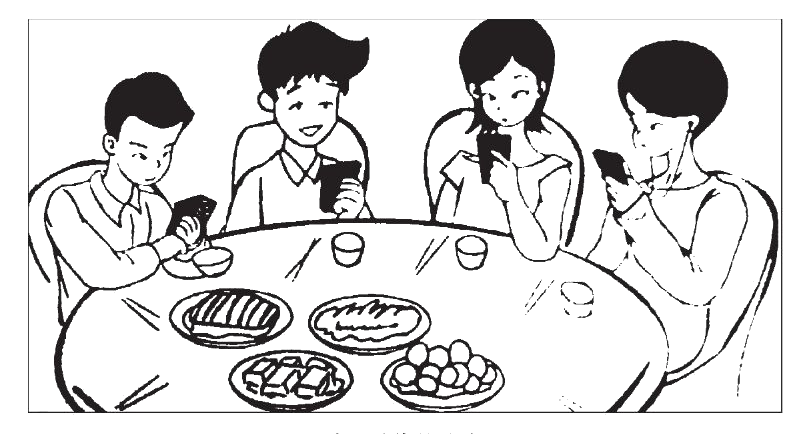
\includegraphics[width=0.58\linewidth]{picture/2015.png}
	\caption*{手机时代的聚会}
\end{figure}

